\documentclass[12pt,journal,a4paper,twoside,onecolumn]{IEEEtran}
\usepackage{amssymb}
\usepackage{mathtools}
\usepackage{ amsmath, bm }
\usepackage{graphicx}
\usepackage{epstopdf}
\usepackage{yhmath}
\DeclareGraphicsExtensions{.pdf,.eps,.png,.jpg,.mps}
\usepackage{dsfont}
\usepackage{bbm}
\usepackage{setspace}
\usepackage[top=1.5in, bottom=1.5in, left=1in, right=1in]{geometry}

%For lemma, theorem, proposition, corllary, proof, definition,example and remark.
\newcommand{\rmnum}[1]{\romannumeral #1}
\newcommand{\Rmnum}[1]{\expandafter\@slowromancap\romannumeral #1@}
\makeatother

\newcommand\bigfrown[2][\textstyle]{\ensuremath{%
  \array[b]{c}\text{\scalebox{2}{$#1\frown$}}\\[-1.3ex]#1#2\endarray}}
% End
\author{An~Jiang,~
        Harry~Leib,~\\
          Department of Electrical Engineering\\
          McGill University\\
          Montreal,~Quebec,~Canada,~\\
          Email: an.jiang@mail.mcgill.ca,~harry.leib@mcgill.ca
}
\title{The Extended Neyman-Pearson Hypotheses Testing Framework and its Application to Spectrum Sensing in Cognitive Wireless Communication}
\date{\today}
\begin{document}
\begin{spacing}{2.5}
\maketitle
\begin{abstract}
Neyman Person (NP) testing for two hypotheses is widely used in radar system, spectrum sensing, medical detection and many other applications. Traditional NP testing maximizes the probability of detection under a probability of false alarm constraint. This paper consider an extended form of the NP test that is suitable for spectrum sensing when there might be different type of primary signals.
\end{abstract}

\begin{IEEEkeywords}
Neyman Pearson, Hypothesis Testing, Spectrum Sensin, Cognitive Radio
\end{IEEEkeywords}

\section{Introduction}
The increasing radio spectrum demand for wireless communication is driving the development of new approaches for its usage, such as Cognitive Radio (CR)\cite{a001}. The concept behind CR networks is the unlicensed use of radio spectrum while ensuring no interference to the licensed users. \cite{goldsmith2009breaking}.
To achieve this goal, a CR system must have ``cognitive" abilities to identify opportunities for communication\cite{buddhikot2007understanding}. In CR systems, the spectrum sensing component brings in such capabilities \cite{tandra2009spectrum}.

 Spectrum sensing has been a subject for extensive studies in the last years\cite{axell2012spectrum}. Common techniques for spectrum sensing are based on energy detection, exploitation of cyclostationarity properties of  the signal being sensed, and also could use preamble sequences that are embedded in the signals \cite{cabric2004implementation}.  In \cite{axell2011optimal}, the authors point out that for OFDM signals when the variances of the noise and signal are known, the performance of energy based spectrum sensing is very close to optimal. Cooperative spectrum sensing \cite{ganesan2005cooperative}, employing multiple sensors that are geographically scattered, are effective against shadowing.
Different sensing algorithms and DSP techniques have been introduced for specific situations, such as in \cite{tian2007compressed} where the authors study algorithms for wide band spectrum sensing focusing on sub-Neyquist sampling techniques. In  \cite{sun2013wideband} and  \cite{sun2013wideband2} the authors propose compressed sensing and sub-Nyquist sampling techniques for wide band spectrum sensing.

In order to detect a free frequency channel, a spectrum sensing scheme solves a binary hypotheses testing problem, where the null hypothesis refers to the event that a user is not using the channel and the alternative hypothesis refers to the event that a user is occupying the channel. If the a-prior probabilities of null and alternative hypotheses are known, then such a problem can be solved using a Bayesian framework \cite{poor1994introduction}. The situation when Baysian framework could be used is considered in \cite{zeng2010review} and the performance of such scheme is analyzed.
Even though the Baysian framework can be used in some situations, in more often cases, the a-prior probabilities are not available. In such situations Neyman Pearson testing is employed \cite{poor1994introduction}.When there is a single type of primary user (two hypotheses), NP testing will achieve the largest probability of detecting a vacant channel when no primary user is present under a constraint on the probability that the channel will be declared vacant when in fact a primary user is present.
Traditional NP testing has been extensively used for two hypotheses problem. In such cases,  the performance is characterized by the Receiver Operating Characteristic (ROC) curve, which represents the relationship between probability of detection and probability of false alarm \cite{poor1994introduction}.

In spectrum sensing application, there may be more than one type of primary users. For example in IEEE 802.22 \cite{shellhammer2008spectrum} the channel can be occupied by Analog-TV Digital-TV and wireless microphone. In such cases, an extended NP (ENP) test can provide important advantages \cite{zhang1999design}. A detector based on ENP testing can ensure the largest probability of detection under a separate constraint of false alarm for each primary user type \cite{LehmannTest}.

With an ENP detector however, the achievable false alarm probabilities are limited. In this work we analyze the properties of the ENP test and propose the Modified Extended Neyman Pearson (MENP) test, that circumvents the limitations of the false alarm probabilities. The structure of the remaining of this paper is [TO BE ADDED].

\section{Extended Neyman Pearson Test}

\subsection{Introduction to Extended Neyman Pearson Test}
The theories of hypotheses testing have been a subject of continuous studies, and have found applications in various fields such as radar systems, spectrum sensing for cognitive communication systems, and in  medical science. One type of hypotheses testing problem can be abstracted as  follows: assume $M+1$  hypotheses $H_0$, $H_1$, ..., $H_{M}$, inducing $M+1$  Probability Density Functions (PDFs) on the observable $Y$.

  \begin{equation}
\label{equ:hypothesis}
\begin{split}
H_0:\;\;\;\;\;\;\;\;\;&Y \sim f_0(y) \\
H_1:\;\;\;\;\;\;\;\;\;&Y \sim f_1(y)\\
&......\\
H_M:\;\;\;\;\;\;\;\;\;&Y \sim f_M(y)\\
\end{split}
\end{equation}
Based on $y$, a realization of $Y$, the detector needs to decide whether or not it comes from $f_0(y)$. A framework for solving this problem for $M=1$ was introduced in \cite{neyman1933problem} and it is commonly known as Neyman Pearson (NP) testing. The theory of NP testing was further developed in \cite{wald1939contributions}. In \cite{dantzig1951fundamental}, the theory of NP testing was  expanded also for $M>2$. A comprehensive exposition of such generalized NP testing can be found in \cite{LehmannTest}.

\noindent  \textbf{The Extended Neyman Pearson (ENP) Lemma:}
\textit{
Let $f_0(x), f_1(x), ..., f_{m}(x)$ be real Borel measurable functions  defined on finite dimensional  Euclidean space $\mathcal{R}$ such that $\int \limits_R | f_i(x)|\mathrm{d}x < \infty (i=0, 1,...,M)$.  Suppose that for given constants $c_1,...,c_M$ there exists a class of subsets $\mathcal{S}$, denoted $\mathcal{C}_\mathcal{S}$, such that for every $\mathcal{S} \in \mathcal{C}_\mathcal{S}$ we have
\begin{equation}
\label{one}
\int\limits_\mathcal{S} f_i(x)\mathrm{d}x = c_i, \;\;\;\;\;\;i=1,...,M
\end{equation}
Then:
%No. 1
\\\textnormal{(\rmnum{1})} Among all members of $\mathcal{C}_\mathcal{S}$ there exists one that maximizes
\[
\int \limits_\mathcal{S} f_{0}(x)\mathrm{d}x.
\]
%No.2
\\\textnormal{(\rmnum{2})} A sufficient condition for a member of $\mathcal{C}_\mathcal{S}$ to maximize
\[
\int \limits_\mathcal{S} f_{0}(x)\mathrm{d}x.
\]
is the existence of constants $k_1,...,k_M$ such that
\begin{equation}
\label{2}
f_{0}(x)>\sum\limits_{j=1}^M k_j f_j(x)\;\;\;\;\text{when $x \in \mathcal{S}$}
\end{equation}
\begin{equation}
\label{3}
f_{0}(x)<\sum\limits_{j=1}^M k_j f_j(x)\;\;\;\;\text{when $x \notin \mathcal{S}$}
\end{equation}
%No. 3
\\\textnormal{(\rmnum{3})} If a member of $\mathcal{C}_\mathcal{S}$ satisfies  \textnormal{(\ref{2})} and \textnormal{(\ref{3})} with $k_1,...,k_M\geq0$, then it maximizes
\begin{equation}
\label{4}
\int \limits_\mathcal{S} f_{0}(x)\mathrm{d}x
\end{equation}
among all $\mathcal{S} \in \mathcal{C}_{\mathcal{S}}$ satisfying
\begin{equation}
\label{5}
\int \limits_\mathcal{S} f_i(x)\mathrm{d}x\leq c_i,\;\;\;\;i=1,...,M.
\end{equation}
}

The associated probability of detection, $P_d$ and false alarms $P_{f_i}$ for a certain subset $\mathcal{S}$ are defined as \cite{neyman1933problem}, $P_d = P(H_0 | H_0) = \int_{\mathcal{S}}f_0(x)\mathrm{d}x, P_{f_i} = P(H_0 | H_i) = \int_{\mathcal{S}}f_i(x)\mathrm{d}x\;\; i = 1, ..., M $. Define the step function

\begin{equation}
   \label{equ: step function}
   u(x) = \begin{cases}
     0\;\;\;\;\;\;&x < 0\\
     0.5\;\;\;\;\;\;&x=0\\
     1\;\;\;\;\;\;&x>0\,,
   \end{cases}
\end{equation}
Then for a subset $\mathcal{S}$ satisfying \eqref{2} and \eqref{3} we have:
\begin{equation}
\label{equ: pf and pd}
\begin{split}
&P_d = \int_{-\infty}^{\infty} u(f_0(x) - \sum_{j=1}^{M}k_jf_j(x)) f_0(x)\mathrm{d}x	\,, \\
&P_{f_i} = \int_{-\infty}^{\infty} u(f_0(x) - \sum_{j=1}^{M}k_jf_j(x)) f_i(x) \mathrm{d}x\;\;	 i=1, 2, ..., M\,.
\end{split}
\end{equation}
The relationship between $P_d$ and $P_{f_i}$ can be represented by Receiver Operating Characteristic (ROC) surface \cite{LehmannTest}.

From to \eqref{2} \eqref{3}, the ENP Decision rule $\delta$ is

\begin{equation}
\label{equ: decision rule}
\delta: \sum_{j=1}^{M}k_j\frac{f_j(x)}{f_0(x)} \substack{H_0 \\ < \\ \geq \\ \bar{H}_0} 1
\end{equation}

From the  \textbf{ENP Lemma}, $\delta$  achieves the largest $P_d$ under the constraints $P_{f_i} = c_i (i = 1, 2, ..., M)$.
When $M=1$, it achieves the largest $P_d$ under the constraint $P_f \leq c$ \cite{LehmannTest}, which is the well known and commonly used form.

% notes from Prof. Leib.
For applications in spectrum sensing, $H_0$ denotes the hypothesis that the channel is free and $H_m \;(m=1, ..., M)$ corresponds to the hypothesis that the channel is occupied by the $m$-th primary signal. Although we have $M$ hypotheses, we intend to determine if the channel is free or not. Hence the problem is to find a binary test of deciding $H_0$ versus $\bar{H}_0$ such that $P_d$ is maximized under the constraints $P_{f_m} \leq c_m$ $m = 1, ..., M$. In context of spectrum sensing, $1-P_{f_m}$ can be interpreted as the protection level of the $m-$th primary signal. The larger is this protection level, the smaller is the probability that when the $m-$th signal is active, the test will not detect it and will declare the channel free. In context of spectrum sensing the solution of the ENP problem maximizes the probability of detecting a free channel under a constraint on the protection level for each primary signal. The protection levels of primary signals can be different and they are guaranteed.

\subsection{Properties of Extended Neyman Pearson Test}
We consider now several properties for the ENP test, embodied by three lemmas with proof placed in the appendix.

\noindent \textbf{Condition 1}
\textit{
\noindent Let $f_i(x) \;\;i=0, 1, ..., M$ be the PDF induced by hypothesis $H_i$, and define $g(x) = f_0(x) - \sum_{j=1}^{M} k_jf_j(x)$ where $k_i$  ($i = 1, 2, ..., M$) are real numbers. Let $\mathcal{D} \in \mathbb{R}$ be an open set such that $\int_{\bar{\mathcal{D}}}f_i(x)=0\;\;i = 1, 2, ..., M$. Furthermore,  if $x_0$ is a solution  for $g(x) = 0 \;\;(x \in \mathcal{D})$, there exists an integer $n$ such that  the $n$ order derivative of $g(x_0)$ is not equal to zero $(g^{(n)}(x_0) \neq 0)$.
}

\noindent \textbf{Lemma 1}
\textit{
\noindent Under}
\textbf{Condition 1}
\textit{, let $\mathbf{P}$ be a point with coordinate $(P_d, P_{f_1}, ..., P_{f_M})$ on the ROC surface of the EPN test. If there exists a tangent hyperplane at $\mathbf{P}$, then its normal is parallel to the vector $\mathbf{n} = (-1, k_1, ..., k_M)$, where $k_i$ are the parameters of the ENP test achieving $\mathbf{P}$.
}

\noindent \textbf{Lemma 2}
\textit{
\noindent
Under}
\textbf{Condition 1}
\textit{, let $\mathbf{P}$ be a point on the ROC surface, $\frac{\partial P_d}{\partial P_{f_i}} \bigg|_P = k_i$, where $k_i$ are the parameters of ENP test achieving $\mathbf{P}$.
}

\noindent \textbf{Lemma 3}
\textit{
\noindent
Under}
\textbf{Condition 1}
\textit{, let $\mathbf{P}$ be a point on the ROC surface. If  $\mathbf{P}$ cannot be achieved by ENP test with all positive parameters, then there  exist another point $\mathbf{P}^\prime\;\; (P_d^\prime, P_{f_1}^\prime, ..., P_{f_M}^\prime)$ on the ROC surface satisfying
}
\begin{equation}
  \label{equ: lemma 3 equation}
  \begin{split}
    P_d^\prime &\geq P_d\\
    P_{f_i}^\prime &\leq P_{f_i}\;\;\;\;i = 1, 2, ..., M\,.
  \end{split}
\end{equation}

\subsection{Modified Extended Neyman Pearson Algorithm}


In practice (e.g. spectrum sensing in CR communication system), the following problem needs to be solved,

      \begin{equation}
      \label{equ: problemstate}
      \begin{split}
      \max\;\;\;\;\;\;&P_d\\
      \text{s.t.}\;\;\;\;\;\;&P_{f_i} \leq c_i\;\;\;\;i = 1, 2, ..., M
      \end{split}
      \end{equation}

According to ENP Lemma, this problem can by solved by ENP test only when there are parameters $k_i \geq 0, \;\;i=1, ..., M$ such that 
\begin{equation}
\label{equ: condition for ENP}
\begin{split}
c_i = \int_{-\infty}^{\infty}u(f_0 - \sum_{j=1}^{M}k_jf_j(x))f_i(x)\mathrm{d}x \;\;i = 1, ..., M
\end{split}
\end{equation}

The case when the given $c_i\;\;i = 1, 2, ..., M$ do not satisfy \eqref{equ: condition for ENP} was not considered so far. Next we present the Modified Extended Neyman Pearson Test (MENP) for solving \eqref{equ: problemstate}.

%define \JUDGEMENT
\def \JUDGEMENT{u(f_0(x) - \sum_{j=1}^{M}k_j f_j(x))}

Define $\mathbf{c}^T = [c_1, c_2, ..., c_M]$, $\mathbf{a}^T=[a_1, a_2, ..., a_M]$, $\mathbf{k}^T = [k_1, k_2, ..., k_M]$ and  $\mathbf{P}_f^T = [P_{f_1}, P_{f_2}, ..., P_{f_M}]$. Let
$F(\mathbf{a})$ denote the largest $P_d$ under the constraints $P_{f_i} = a_i\;\;i = 1, ..., M$.
Also define the set $\mathcal{A}_\mathbf{c} = \{
  \mathbf{P}_f | 0 \leq P_{f_i} \leq c_i
  \;\;i=1, 2, ..., M\}\,.
$ and set $\alpha^+ \triangleq \{\mathbf{P}_f | P_{f_i} = \int_{-\infty}^{\infty} \JUDGEMENT f_i(x) \mathrm{d}x, \text{where\;\;} k_i \geq 0 \;\;i=1, ..., M\}$.

\noindent \textbf{Modified Extended Neyman Pearson test}

\noindent \textit{
If \textnormal{\textbf{Condition 1}} is satisfied, then:
\\\textnormal{(\rmnum{1})} Assume $\mathbf{c} \in \alpha^+$. Then there must be a $\mathbf{k}^0 = [k_1^0, k_2^0, ..., k_M^0]^T$ with $k_i \geq 0\;\;i=1, ..., M$ satisfying
}
\begin{equation}
\label{equ:Pf}
  P_{f_i}^0 = \int_{-\infty}^{\infty} u(f_0(x) - \sum_{j=1}^{M}k_j^0f_j(x))f_i(x)\mathrm{d}x = c_i \;\; (i= 1, 2, ..., M)\,.
\end{equation}
\textit{
and the decision rule $\delta $ solving  \eqref{equ: problemstate} is:
}
\begin{equation}
\label{equ:decision rule}
\delta:\;\;\;\;\frac{f_0(x)}{\sum_{i=1}^{M}k_i^0f_i(x)} \substack{H_0 \\ \geq \\ < \\ \bar{H}_0} 1
\end{equation}
\textit{
\noindent \textnormal{(\rmnum{2})} Assuming $\mathbf{c} \notin \alpha^+$, Let $\mathcal{C} = \mathcal{A}_{\mathbf{c}} \cap \alpha^+$, and $\mathbf{a}^0 = [a_1^0, a_2^0, ..., a_M^0]^T \in \mathcal{C}$ be such that
}
\begin{equation}
\label{equ: F0}
\max_{\mathbf{a} \in \mathcal{C}}\;\;\;\;F(\mathbf{a}) = F(\mathbf{a}^0)\\
\end{equation}
\textit{
Since $\mathbf{a}^0 \in \mathcal{A}_{\mathbf{c}} \cap \alpha^+$, from \textnormal{(\rmnum{1})} we have that there exists a vector $\mathbf{k}^0$ such that}  \eqref{equ:decision rule} \textit{ maximizes $P_d$ under the constraints $P_{f_i} = a_i^0, \;i=1, ..., M$. Here since $a_i^0 \leq c_i^0, \;i=1, ..., M$ this decision rule  solves} \eqref{equ: problemstate}.

Next we introduce a method of finding $\mathbf{a}^0$ in (\rmnum{2}). 
Since when $\mathbf{a} \in \alpha^+$ we have 
\begin{equation}
  \begin{split}
    \underset{\mathbf{a} \in \alpha^+}{\max}\;\;\;\;&P_d = F(\mathbf{a})\\
    \text{s.t.}\;\;\;\;&P_{f_i} = a_i\;\;\;i=1, ..., M\,,
  \end{split}
\end{equation}
According to ENP Lemma, $F(\mathbf{a})$ also satisfies
\begin{equation}
  \begin{split}
  \label{equ: F}
        \underset{\mathbf{a} \in \alpha^+}{\max}\;\;\;\;&P_d = F(\mathbf{a})\\
    \text{s.t.}\;\;\;\;&P_{f_i} \leq a_i\;\;\;i=1, ..., M\,.
  \end{split}
\end{equation}

In \eqref{equ: F}, when one of $a_i, i = 1, ..., M$ increases and other $a_i$ remain the same, the constraints is more relaxed, so $P_d$ will not decrease. Therefore $F(\mathbf{a})$ is a non-decreasing function of $a_i\;\;(i = 1, ..., M)$ when $\mathbf{a} \in \alpha^+$. Hence we can conclude $\mathbf{a}^0$ has the largest components $a_i^0$ among all $\mathbf{a} \in \mathcal{C}$. 
[TO BE ADDED]
When trying to find $\mathbf{a}^0$, we only need to iterate $\mathbf{a} \in \alpha$ who have the largest components $a_i$.

From (\rmnum{1}) and (\rmnum{2}), it can also be concluded that for any given $(c_1, c_2, ..., c_M)$, the decision rule has form  \eqref{equ: decision rule} with $k_i \geq 0\;\;i=1, ..., M$.

The proof that MENP achieves the optimal decision rule is given in the appendix.

\section{The ROC surface of MENP}

The ROC surface of MENP (M-ROC) depicts the relationship between $P_d$ and $c_1, c_2, ..., c_M$. On one hand, it  illustrates the largest $P_d$ can that can be achieved under the constraints $P_{f_i} \leq c_i (i = 1, 2, ..., M)$, on the other hand, it provides the range of $\mathbf{c}$ for a given $P_d$.
Points $(P_d, c_1, c_2, ..., c_M)$ on M-ROC  surface can be divided into two types: 
\\1. Those with $[c_1, c_2, ..., c_M] \in \alpha^+$. Define this set of points as $M_0$; 
\\2. Those with $[c_1, c_2, ..., c_M] \notin \alpha^+$. Define this set of points as $M_1$. 

Obviously points in $M_0$ can be achieved by MENP (\rmnum{1}) and points in $M_1$ can  be achieved by MENP (\rmnum{2}). Next we consider a property of the M-ROC surface.

\noindent\textbf{Property 1}

\noindent  \textit{
\noindent For a given $\alpha \in [0,1)$, an M-ROC surface segment with points satisfying $P_d \geq \alpha$ is  convex.
}

\noindent \textbf{Property 2}
\noindent \textit{The boundary point of set $\alpha^+$ can be achieved by decision rule}
\begin{equation}
\label{equ: boundary decision rule}
\frac{f_0(x)}{\sum_{i=1}^{M}k_if_i(x)} \substack{H_0 \\ \geq \\ < \\ \bar{H}_0} 1 
\end{equation}
where at lease one $k_s$ ($s$ is an integer between $1$ and $M$) is zero. 

\noindent \textbf{Property 3}

\noindent \textbf{Property 4}
\noindent \textit{
  \noindent Assume hypotheses given as:
}
\begin{equation}
\begin{split}
H_0:\;\;\;\;\;\;&X \sim f_0(x)\\
H_1:\;\;\;\;\;\;&X \sim f_1(x)\\
  &......\\
H_M:\;\;\;\;\;\;&X \sim f_M(x)
\end{split}
\end{equation}
\textit{
  define $g(x) = \frac{\sum_{i=1}^{M}k_if_i(x)}{f_0(x)}$. If $g(x)$ is a monotonically increasing function of $x$ for any non-negative $k_i\;\;(i = 1, ..., M)$ and $F_i(x)$, which is the CDF of hypotheses $H_i (i = 0, ..., M)$, is monotonically increasing function, then we have:}
  
\textit{(1)The region $M_0$ degenerates to a curve and the decision rule for $M_0$ is $x \substack{\bar{H}_0 \\ \geq \\ < \\H_0} x_0$.}

\textit{(2)For a specific false alarm constraints $P_{f_i} \leq c_i\;\;(i = 1, ..., M)$, the decision rule for MENP test is $x \substack{\bar{H}_0 \\ \geq \\ < \\H_0} x_0$, where $x_0 = \min(F_i^{-1}(c_i))\;\;i = 1, ..., M$.}

\textit{(3)The expression of $P_d$, $P_{f_1}$, ..., $P_{f_M}$ can be written as}
\begin{equation}
\label{equ: chi pd}
  \begin{split}
    P_d &= \text{Pr}(X \leq x_0 | H_0) = F_0(x_0)\\
        P_{f_1} &= \text{Pr}(X \leq x_0 | H_1) = F_1(x_0)\\
        &......\\
            P_{f_M} &= \text{Pr}(X \leq x_0 | H_2) = F_M(x_0)
  \end{split}
\end{equation}

The proof is given in the appendix.

Next we consider two examples that illustrate the properties of M-ROC surface for $M = 2$.

\subsection{Gaussian Hypotheses}
Assume three hypotheses given as:
\begin{equation}
\label{equ: Gaussian Hypothesis}
\begin{split}
	H_0:\;\;\;\;\;\;\;\;&X \sim \mathcal{N}(-1,1)\\
    H_1:\;\;\;\;\;\;\;\;&X \sim \mathcal{N}(0,1)\\
    H_2:\;\;\;\;\;\;\;\;&X \sim \mathcal{N}(1,10)\,,
\end{split}
\end{equation}
where $\mathcal{N}(\mu,\sigma^2)$ denotes a Gaussian PDF with mean $\mu$ and variance $\sigma^2$.
To form the M-ROC surface, we first consider points in region $M_0$.The decision rule in region $M_0$ is given by \eqref{equ: decision rule}
with $M=2,\;\;k_1, k_2 \geq 0$, and the expression for $P_d$, $P_{f_1}$ and $P_{f_2}$ are given by \eqref{equ: pf and pd}. According to \textbf{Neyman Pearson Lemma}, if $k_1, k_2 \geq 0$, then $P_{f_1} = c_1$ and $P_{f_2} = c_2$.

We use Matlab to illustrate the region $M_0$. The values of $k_1$ and $k_2$ range from $0$ to $100$ in steps of $0.01$. Substituting the value of $k_1$ and $k_2$ into \eqref{equ: pf and pd}, results in the corresponding $P_d$ $P_{f_1}$ and $P_{f_2}$.  The set $M_0$ is illustrated in Figure \ref{pic: surface for m0 gaussian}. Figure \ref{pic: contour for m0 gaussian} presents the projection of Figure \ref{pic: surface for m0 gaussian} on the $c_1, c_2$ plane.
In Figure \ref{pic: contour for m0 gaussian}, region $N_0$ is the projection of region $M_0$ on the $c_1, c_2$ plane. Since $M_0$ is the set of points with $[c_1, c_2] \in \alpha^+$, $N_0$ is the region of points that belong to $\alpha^+$.
Define curve $L_1$ as the set of points that satisfy the conditions: (1) $(c_1, c_2) \in N_0$; (2) $(c_1, c_2+\epsilon) \notin N_0$, for any $\epsilon \geq 0$. Define curve $L_2$ as the set of points that satisfy the conditions: (1) $(c_1, c_2) \in N_0$; (2) $(c_1 + \epsilon, c_2) \notin N_0$, for any $\epsilon \rightarrow 0$.
$N_1$ denotes the region enclosed by line $c_1 = 0$, $c_2$; line $c_1$, $c_2 = 1$ and curve $L_1$.
$N_2$ denotes the region enclosed by line $c_1 = 1$, $c_2$; line $c_1$, $c_2 = 0$ and curve $L_2$.
The regions of $N_0$ $N_1$ and $N_2$ are shown in Figure \ref{pic: contour for m0 gaussian}.

\textbf{Conclusion 1}
\textit{\\(1) All points belonging to region $N_1$ or curve $L_1$, if they have the same $c_1$, they have the same decision rule and same $P_d$.
\\(2) All points belonging to region $N_2$ or curve $L_2$, if they have the same $c_2$, they have the same decision rule and same $P_d$.
}

The proof is given in the appendix.

Since we already know $P_d$ for points in region $N_0$ and curves $L_1$ and $L_2$ belong to $N_0$, we can get $P_d$ for points in $N_1$ and $N_2$. M-ROC surface for this example is given in Figure  \ref{pic: LJS} and the contour of M-ROC surface is given in Figure \ref{pic: LJS contour}.

Next we consider a more general case of $M+1$ hypotheses given as
\begin{equation}
\label{equ: m+1 Gaussian Hypo}
\begin{split}
H_0:\;\;\;\;\;\;&X\sim \mathcal{N}(\mu_0, \sigma_0^2)\\
H_1:\;\;\;\;\;\;&X\sim \mathcal{N}(\mu_1, \sigma_1^2)\\
  ......\\
H_M:\;\;\;\;\;\;&X\sim \mathcal{N}(\mu_M, \sigma_M^2)
\end{split}
\end{equation}
We will prove when $\sigma_0^2 = \sigma_1^2 = ... = \sigma_M^2$ and $\mu_0 < \mu_i (i = 1, ..., M)$, the region achieved by ENP test with $k_i \geq 0 (i = 1, ..., M)$ degenerates to a curve.

Consider
\begin{equation}
\label{equ: define gx}
g(x) = \sum_{i=1}^{M}k_i\frac{f_i(x)}{f_0(x)}.
\end{equation}
Since 
\begin{equation}
\label{equ: gaussian PDF}
f_i(x) = \frac{1}{\sqrt{2\pi\sigma_i^2}}\exp(-\frac{(x-\mu_i)^2}{2\sigma_i^2}).
\end{equation}
we have
\begin{equation}
\label{g00}
g(x) = \sum_{i=1}^{M}\frac{\frac{1}{\sqrt{2\pi\sigma_i^2}}\exp(-\frac{(x-\mu_i)^2}{2\sigma_i^2})}{\frac{1}{\sqrt{2\pi\sigma_0^2}}\exp(-\frac{(x-\mu_0)^2}{2\sigma_0^2})}
\end{equation}
Using the condition $\sigma_i^2 = \sigma_0^2 (i = 1, ..., M)$ in \eqref{g00}, we have 
\begin{equation}
\label{equ: gx cc}
g(x) = \sum_{i=1}^{M}k_i\exp(\frac{(\mu_i - \mu_0)(2x-\mu_i - \mu_0)}{2\sigma_0^2})
\end{equation}
Defining $c_i = \frac{\mu_i - \mu_0}{2\sigma_0^2}$, \eqref{equ: gx cc} can be written as
\begin{equation}
g(x) = \sum_{i=1}^{M}k_i\exp(c_i(2x-\mu_0 - \mu_i)
\end{equation}
From the condition $\mu_0 < \mu_i (i=1, ..., M)$, we know $c_i >0$. Hence it can be conclude that $g(x)$ is a monotonically increasing function with $x$. Hence from \textbf{Property 4} we have that the region $M_0$ (region achieved by ENP test with $k_i \geq 0 (i=1, ..., M)$) degenerates to a curve.

%different subsection
\subsection{Chi-Square Hypotheses}
Assume three hypotheses  given as:
\begin{equation}
  \label{equ: Chisquare Hypothesis}
  \begin{split}
    H_0:\;\;\;\;\;\;\;\;&\frac{X}{\sigma_0^2} \sim \mathcal{X}^2(2N)\\
    H_1:\;\;\;\;\;\;\;\;&\frac{X}{\sigma_1^2} \sim \mathcal{X}^2(2N)\\
    &......\\
    H_M:\;\;\;\;\;\;\;\;&\frac{X}{\sigma_2^M} \sim \mathcal{X}^2(2N)\,,
  \end{split}
\end{equation}
where $\mathcal{X}^2(2N)$ is the Chi-square distribution with  $2N$ degree freedom($N$ is an integer, $\sigma_0^2 < \sigma_1^2, ..., \sigma_M^2$ and $\sigma_i^2 \neq \sigma_j^2$ if $i \neq j$). By a random variable transformation space \cite{mark2011probability}, we can get the PDFs for the hypotheses:

\def \CHISQU[#1]{\frac{1}{#1 2^N\Gamma(N)}\left(\frac{x}{#1}\right)^{N-1}\exp\left(-\frac{x}{2#1}\right)\\}
\begin{equation}
  \label{equ: Chisquare Distribution}
  \begin{split}
    H_0:\;\;\;\;\;\;\;\;&f_0(x) = \CHISQU[\sigma_0^2]\\
    H_1:\;\;\;\;\;\;\;\;&f_1(x) = \CHISQU[\sigma_1^2]\\
    &......\\
    H_M:\;\;\;\;\;\;\;\;&f_2(x) = \CHISQU[\sigma_M^2]\,.
  \end{split}
\end{equation}

In the following, we will prove that in this example the region achieved by ENP test with $k_i \geq 0 (i = 1, ..., M)$ degenerates to a curve.

Consider
\begin{equation}
\label{equ: decision rule chi}
  g(x) = \frac{\sum_{i=1}^{M}k_if_i(x)}{f_0(x)} \;\;\;\;k_i \geq 0
\end{equation}
Substituting $f_i(x) (i=1, ..., M)$ from \eqref{equ: Chisquare Distribution} into \eqref{equ: decision rule chi}, we get:

\begin{equation}
  \label{equ: decision rule chi 1}
g(x) = \sum_{i=1}^{M}k_i'\exp{(\frac{1}{2\sigma_0^2} - \frac{1}{2\sigma_i^2})x} 
\end{equation}
where $k_i' = k_i(\frac{\sigma_0}{\sigma_i})^{2N}, i= 1, ..., M$. Define $p_i = \frac{1}{2\sigma_0^2} - \frac{1}{2\sigma_i^2}, i=1, ..., M$. Hence $g(x) =  \sum_{i=1}^{M}k_i'\exp{p_ix}$.

The parameters $k_i' (i=1, ..., M)$ are always non-negative when $k_i (i=1, ..., M)$ are such, and from 
 the condition $\sigma_0^2 \leq \sigma_i^2 (i=1, ..., M)$ we can conclude $p_i (i=1, ..., M)$ are positive. Hence $g(x)$ is a monotonically increasing function with $x$. From \textbf{Property 4}, we have that the region achieved by ENP test with $k_i (i = 1, ..., M)$ degenerates to a curve and the decision rule is
\begin{equation}
  \label{equ: decision rule chi 2}
  x \substack{\bar{H}_0 \\ \geq \\ < \\ H_0} x_0\;\;\;\;\,.
\end{equation}

Since under Chi-Square distribution, $f_i(x) =0 (i = 0, 1, ..., M)$ if $x<0$, we can conclude $x_0 \geq 0$.

In the following, an example for Chi-Square Hypotheses with $M=2$, $\sigma_0^2 = 1$, $\sigma_1^2 = 1.1$, $\sigma_2^2 = 1.15$ and $N=120$ is given.

To form the M-ROC surface, we first consider points in region $M_0$ ($(c_1, c_2) \in \alpha$). As we have proved, the decision rule for this region is $x \substack{\bar{H}_0 \\\geq\\< \\ H_0 } x_0 (x_0 \geq 0)$ and the expression of $P_d$ $P_{f_1}$ $P_{f_2}$ can be derived by \eqref{equ: chi pd}.  According to Extended NP test, when $k_1, k_2 \geq 0$, we have $P_{f_1} = c_1$ and $P_{f_2} = c_2$. Hence $c_1$, $c_2$ and $P_d$ can be derived by
\begin{equation}
\begin{split}
P_d &= F_0(x_0)\\
c_1 &= F_1(x_0)\\
c_2 &= F_2(x_0)\,.
\end{split}
\end{equation}

By using \textbf{Conclusion 1}, we can derive the $P_d$ for $(c_1, c_2) \notin \alpha^+$.
The M-ROC surface is plotted in Figure \ref{pic: LJS for chisquare}.Since for points $(c_1, c_2) \in \alpha$, the decision rule is  $x \substack{\bar{H}_0 \\\geq\\< \\ H_0 } x_0 (x_0 \geq 0)$, according to \textbf{Conclusion 1}, we can conclude that for $(c_1, c_2) \notin \alpha^+$, the M-ENP decision rule also has the form of $x \substack{\bar{H}_0 \\\geq\\< \\ H_0 } x_0 (x_0 \geq 0)$.  
\section{Energy Based Spectrum Sensing for two Primary Users}
In this section, we consider an example for applying the MENP test to energy based spectrum sensing for two primary users.

\subsection{System Model}
Consider a cognitive radio system where the frequency can be occupied by one of the two  distinct primary signals $\{ s_1, s_2 \}$ or it could be vacant.
Let  $H_0$  denote the hypothesis that the channel is vacant, and $H_i, i = 1, 2$, denote the hypothesis that the channel is occupied by primary user signal $s_i, i=1, 2$. We test $H_0$ against $\overline{H}_0$ using the ENP framework. The problem can be abstracted into following optimization problem:
\begin{equation}
  \label{equ: energy spectrum sensing}
  \begin{split}
  \max \;\;\;\;\;\;\;\;\;\;\;\;\;\;\; &P_d\,,\\
  \text{s.t.} \;\;\;\;\;\;\;\;\;\;\;\;\;\;\; &P_{f_i} \leq c_i\;\;\;\;(i = 1, 2)\,.
  \end{split}
\end{equation}

Our object is to plot the maximum $P_d$ vs. $c_1, c_2$ (M-ROC) and find the specific decision rule for a given $c_1, c_2$.

A block diagram of the system is illustrated in Figure \ref{pic: block diagram}. The system consists of a measuring device followed by a testing device. The role of the measuring device is to output a suitable test statistics. The role of the testing device is to decide whether the channel is free based on the output of the measuring device. The input of the measuring device is

\begin{equation}
  \label{equ: expression of x}
  x[n]=\begin{cases}
    \omega[n]\;\;\;\;\;\;\;\;\;\;\;\;\;\;&\text{when no primary user is occupying the channel}\\
    \omega[n] + s_i[n]\;\;&\text{when primary user $i$ is occupying the channel}\,.
  \end{cases}
\end{equation}
for $n = 1, 2, ..., N$, and $i = 1, 2$. We also assume that $s_i[n]$ and $\omega[n]$ are i.i.d. circular symmetric complex Gaussian(CSCG) random variables with variance $2\sigma_{s_i}^2$ and $2\sigma_{\omega}^2$, in other words, $s[n] \sim \mathcal{CN}(0, 2\sigma_{s_i}^2) $ and $\omega[n] \sim \mathcal{CN}(0, 2\sigma_\omega^2)$. Since the noise and the signal are independent, $s_i[n] + \omega[n] \sim \mathcal{CN}(0, 2(\sigma_\omega^2 + \sigma_{s_i}^2))$.

When the testing device is a energy detector, its output is
\begin{equation}
  \label{equ: output of energy detector}
  X = \sum_{n=1}^{N}|x[n]|^2 = \sum_{n=1}^{N}(x_R[n]^2+x_I[n]^2)\,,
\end{equation}
where $x_R$ and $x_I$ are the real and imaginary part of signal $x$. Substituting \eqref{equ: expression of x} into \eqref{equ: output of energy detector} and defining $\sigma_{i}^2 = \sigma_\omega^2 + \sigma_{s_i}^2$ we have

  \begin{equation}
   \label{v3eq7}
   \begin{split}
     \mathcal{H}_0:\;\;\;\;\;\;&\frac{X}{\sigma_\omega^2} \sim \mathcal{X}_{2N}\\
     \mathcal{H}_1:\;\;\;\;\;\;&\frac{X}{\sigma_1^2} \sim \mathcal{X}_{2N}\\
     \mathcal{H}_2:\;\;\;\;\;\;&\frac{X}{\sigma_{2}^2} \sim \mathcal{X}_{2N}
     \end{split}
 \end{equation}

Since $\sigma_\omega^2 < \sigma_1^2, \sigma_2^2$, this problem has the same form as that of the Chi-Square example given in last section.
Hence we can conclude that for any given $c_1, c_2$ the decision rule has the form
\begin{equation}
\label{equ: decision rule for spectrum sensing}
\delta:\;\;\;\;\;\;\;\; x \substack{H_0 \\ \leq \\ > \\\bar{H}_0} x_0\,,
 \end{equation}
where $x_0 = \min(F_1^{-1}(c_1), F_2^{-1}(c_2))$.

\section{Conclusions}
In this paper, we explore the new field of spectrum sensing with emphasis on providing different levels of protections for various primary users. 
The proposed MENP test could achieve the largest probability of detection detection under multiple constraints of probability of false alarms. 
After that, we approach M-ROC surface to represent the relationship between the probability of detection and the constraint conditions. Two examples respectively concerning Gaussian distribution and Chi-Square distribution are given to show the properties of M-ROC surface. 
We also proposed an energy based detector for two different types of primary users.
For simplicity, we assume the signal samples of the primary users subject to iid CSCG distribution and the variance of the signal and the noise are known to the detector.
By simulation, we showed the performance of this detector. 
In this work we assume the detector has the information of the signals' variance. There are other ways dealing with unknown parameters, for example using cyclostationary property to estimate the variance of the primary users. This could be a future topic.  

\appendix
\subsection{Proof for Lemma 1}

Define $\mathbf{k} = [k_1, k_2, ..., k_M]^T$ and $\mathbf{P}_f = [P_{f_1}, P_{f_2}, ..., P_{f_M}]^T$. Since both $P_d$ and $\mathbf{P}_f$ are functions of $\mathbf{k}$, $\mathbf{P}_f(\mathbf{k}_0)$ denotes the value of $\mathbf{P}_f$ when $\mathbf{k} = \mathbf{k}_0$ and $P_d(\mathbf{k}_0)$ denotes the value of $P_d$ when $\mathbf{k} = \mathbf{k}_0$. Using Taylor's expansion for $\mathbf{P}_f$ and $P_d$,
\begin{equation}
\label{pro: pd}
P_d = P_d(\mathbf{k}_0) + \frac{\mathrm{d}P_d}{\mathrm{d}\mathbf{k}^T}\bigg{|}_{\mathbf{k}=\mathbf{k_0}}(\mathbf{k} - \mathbf{k}_0)
+ o(\mathbf{k} - \mathbf{k}_0)
\end{equation}

\begin{equation}
\label{pro: pf}
\mathbf{P}_f = \mathbf{P}_f(\mathbf{k}_0) + \frac{\mathrm{d}\mathbf{P}_f}{\mathrm{d}\mathbf{k}^T}\bigg{|}_{\mathbf{k}=\mathbf{k_0}}(\mathbf{k} - \mathbf{k}_0)
+ o(\mathbf{k} - \mathbf{k}_0)
\end{equation}
here $\mathbf{k} \rightarrow \mathbf{k}_0$.

Consider the hyperplane $y$ as a function of $\mathbf{x}$ defined by
\begin{equation}
\label{pro: x}
\mathbf{x} = \mathbf{P}_f(\mathbf{k}_0) + \frac{\mathrm{d}\mathbf{P}_f}{\mathrm{d}\mathbf{k}^T}\bigg{|}_{\mathbf{k}=\mathbf{k_0}}(\mathbf{z} - \mathbf{k}_0)
\end{equation}
\begin{equation}
\label{pro: y}
y = P_d(\mathbf{k}_0) + \frac{\mathrm{d}P_d}{\mathrm{d}\mathbf{k}^T}\bigg{|}_{\mathbf{k}=\mathbf{k_0}}(\mathbf{z} - \mathbf{k}_0)
\end{equation}
The above equations construct a tangent hyperplane for the ROC surface at point $(P_d(\mathbf{k}_0), \mathbf{P}_f^T(\mathbf{k}_0))$. Combining both equations  we get

\begin{equation}
\label{pro : y2}
y = P_d(\mathbf{k}_0) + \frac{\mathrm{d}P_d}{\mathrm{d}\mathbf{k}^T}\bigg{|}_{\mathbf{k}=\mathbf{k_0}}(
\frac{\mathrm{d}\mathbf{P}_f}{\mathrm{d}\mathbf{k}^T}\bigg{|}_{\mathbf{k}=\mathbf{k_0}}
)^{-1} (\mathbf{x} - \mathbf{P}_f(\mathbf{k}_0))
\end{equation}
Hence the normal for point $(P_d(\mathbf{k}_0), \mathbf{P}_f^T(\mathbf{k}_0))$ on ROC surface can be written as
\begin{equation}
\label{vec: normal}
[-1, \frac{\mathrm{d}P_d}{\mathrm{d}\mathbf{k}^T}\bigg{|}_{\mathbf{k}=\mathbf{k_0}}(
\frac{\mathrm{d}\mathbf{P}_f}{\mathrm{d}\mathbf{k}^T}\bigg{|}_{\mathbf{k}=\mathbf{k_0}}
)^{-1}
].
\end{equation}

In the following, we will prove $ \frac{\mathrm{d}P_d}{\mathrm{d}\mathbf{k}^T}(
\frac{\mathrm{d}\mathbf{P}_f}{\mathrm{d}\mathbf{k}^T}
)^{-1} = \mathbf{k}^T
$, which can be written as
\begin{equation}
\label{pro: vec}
\frac{\mathrm{d}P_d}{\mathrm{d}\mathbf{k}^T} = \mathbf{k}^T \frac{\mathrm{d}\mathbf{P}_f}{\mathrm{d}\mathbf{k}^T}
\end{equation}

Previous equation can be written in component form as
\begin{equation}
\label{pro: component}
\frac{\partial P_d}{\partial k_i} - \sum_{n=1}^{M}k_n\frac{\partial P_{f_n}}{\partial k_i} = 0 \;\;\;\;(i=1, 2, ..., M).
\end{equation}
Calculating the  partial derivatives results in
\begin{equation}
\label{pro: Pf par k}
\frac{\partial P_{f_n}}{ \partial k_i} = - \int_{\mathcal{D}}\delta (f_0(x) - \sum_{j=1}^{M}k_jf_j(x))f_i(x)f_n(x) \mathrm{d}x\,,
\end{equation}
\label{pro: Pd par k}
\begin{equation}\frac{\partial P_d}{ \partial k_i} = - \int_{\mathcal{D}}\delta (f_0(x) - \sum_{j=1}^{M}k_jf_j(x))f_i(x)f_0(x) \mathrm{d}x\,,
\end{equation}
where $\delta(\bullet)$ is Dirac's delta function defined as following,

\begin{equation}
\label{pro: delta}
\delta(x) = \substack{\lim \\ \epsilon \rightarrow 0} \begin{cases}
\frac{1}{\epsilon}\;\;\;\;&\text{when} \;\;x \in (-\frac{\epsilon}{2}, \frac{\epsilon}{2})\\
0\;\;\;\;&\text{otherwise}
\end{cases} \;\;\;\;
\end{equation}

Defining $g(x) = f_0(x) - \sum_{j=1}^{M} k_jf_j(x)$, \eqref{pro: component} can be written as $\int_{\mathcal{D}}\delta(g(x))g(x)f_n(x)\mathrm{d}x = 0, n = 0, 1, ..., M$.

When $g(x) \neq 0$, we have $\delta(g(x)) = 0$ and $\delta(g(x))g(x)f_i(x) = 0$.   When  $g(x) = 0$, we can solve the equation according to the definition of $\delta(\bullet)$ and consider
\begin{equation}
\label{pro: important}
\int_{\{x|g(x)\in (-\frac{\epsilon}{2}, \frac{\epsilon}{2})\}} \frac{1}{\epsilon} g(x)f_n(x) \mathrm{d}x\;\;\;\;n=0, 1, ..., M
\end{equation}

Since when $g(x) \in (-\frac{\epsilon}{2}, \frac{\epsilon}{2})$, $|g(x)| < \frac{\epsilon}{2}$,
\begin{equation}|
\int_{\{x|g(x)\in (-\frac{\epsilon}{2}, \frac{\epsilon}{2})\}} \frac{1}{\epsilon} g(x)f_i(x) \mathrm{d}x | <
\int_{\{x|g(x)\in (-\frac{\epsilon}{2}, \frac{\epsilon}{2})\}} \frac{1}{2}f_i(x) \mathrm{d}x
\end{equation}

Assume $x_s$ is one of the zero point of $g(x)$, also assume $g^\prime(x_s)$, $g^{(2)}(x_s)$, ..., $g^{(n-1)}(x_s)$ are zero but $g^{(n)}(x_s) \neq 0$ (here $n = 1, 2, ...$). Use Taylor expansion near point $x_s$,
\begin{equation}
  \label{equ: gx taylor expansion}
  g(x) = \frac{g^{(n)}(x_s)}{n!}(x - x_s)^n + o((x - x_s)^n)\,.
\end{equation}
%define
\def \LEFT{ x_s
  -\left(\frac{n!\varepsilon}{2|g^{(n)}(x_s)|}\right)^{\frac{1}{n}}}
  \def \RIGHT{ x_s
  +\left(\frac{n!\varepsilon}{2|g^{(n)}(x_s)|}\right)^{\frac{1}{n}}}
%end define
From equation \eqref{equ: gx taylor expansion}, it can be seen when $g(x)\in (-\frac{\epsilon}{2}, \frac{\epsilon}{2})$, $x \in \left(
      \LEFT, \RIGHT
  \right)$.  Define $\bigtriangleup x = \left(\frac{n!\varepsilon}{2|g^{(n)}(x_s)|}\right)^{\frac{1}{n}}$, when $\epsilon \rightarrow 0$, $\bigtriangleup x \rightarrow 0$ and
\begin{equation}
\label{pro: scale}
g(x) \in (-\frac{\epsilon}{2}, \frac{\epsilon}{2})  \Leftrightarrow x \in (x_s -\bigtriangleup x, x_s + \bigtriangleup x)
\end{equation}
 Hence when $\epsilon \rightarrow 0$ we have
\begin{equation}
\int_{\{x|g(x)\in (-\frac{\epsilon}{2}, \frac{\epsilon}{2})\}} \frac{1}{2}f_i(x) \mathrm{d}x \rightarrow
f_i(x_s)\bigtriangleup x \rightarrow 0
\end{equation}

Using the above two conclusions for $g(x) = 0$ and $g(x) \neq 0$, we get
\begin{equation}
\int_{\mathcal{D}} \delta (g(x)) g(x)f_i(x) \mathrm{d}x = 0
\end{equation}

In this way, we prove the normal for the point \textbf{P} on the ROC is $(-1, k_1, k_2, ..., k_M)$.

\subsection{Proof for Lemma 2}
The expression of tangent hyper surface for point $(P_d^0, P_{f_1}^0, ..., P_{f_M}^0)$ on the ROC hyper surface can be written as
\begin{equation}
P_d = P_d^0 + \sum_{i=1}^{M} \frac{\partial P_d}{\partial P_{f_i}}\bigg|_{P_{f_i} = P_{f_i}^0}(P_{f_i} - P_{f_i}^0)\,.
\end{equation}
Hence the normal at this point is

 $\mathbf{n} = [-1, \frac{\partial P_d}{\partial P_{f_1}}, \frac{\partial P_d}{\partial P_{f_2}}, ..., \frac{\partial P_d}{\partial P_{f_M}}]$. Since we have proved that  the normal for this point is $\mathbf{n} = [-1, k_1, k_2, ..., k_M]$, we must have
\begin{equation}
\frac{\partial P_d}{\partial P_{f_i}}\bigg|_{P} = k_i
\end{equation}


\subsection{Proof for Lemma 3}
Assume $\mathbf{P} (P_d, P_{f_1}, ..., P_{f_M})$ is a point on the ROC and it cannot be achieved by ENP test with non-negative parameters. Assume it can be achieved by ENP test with parameter $\mathbf{k} = [k_1, k_2, ..., k_M]^T$ and $k_l$ is negative.

 If there exists a tangent hyper plane at point $\mathbf{P}$, according to \textbf{Lemma 2}, $\frac{\partial P_d}{\partial P_{f_l}} = k_l < 0$. Consider another point $\mathbf{P}' (P_d', P_{f_1}', ..., P_{f_M}')$, here $P_{f_i} = P_{f_i}' (i \neq l)$ and $P_{f_l}' = P_{f_l} - \epsilon \;\;(\epsilon \rightarrow 0 \text{and} \epsilon >0)$. The partial derivative can be written in following form:
 \begin{equation}
   \frac{\partial P_d}{ \partial P_{f_l}} \bigg|_{\mathbf{P}} = \frac{P_d - P_d'}{P_{f_l} - P_{f_l}'} = k_l\,.
 \end{equation}
 Hence
 \begin{equation}
   P_d - P_d' = \epsilon k_l
 \end{equation}
 The expression of $P_d'$ can be written as
 \begin{equation}
   P_d'= P_d - \epsilon k_l\,.
 \end{equation}
Since $k_l < 0$, $P_d' > P_d$. By comparing $\mathbf{P}'$ with $\mathbf{P}$, we can conclude
\begin{equation}
\begin{split}
  P_{d}^\prime &> P_{d}^0\\
  P_{f_i}^\prime &\leq P_{f_i}^0 \;\;\;\;\;\;\;\;\text{for}\;\;\;\;\;\; i=1, 2, ..., M\,.
\end{split}
\end{equation}

If there is no tangent hyper plane at point $\mathbf{P}$, we use another point to approximate $\mathbf{P}$. 
Assume $\mathbf{P}' (P_d', P_{f_1}', ..., P_{f_M}')$ is a point achieved by ENP parameters $\mathbf{k}=[k_1', k_2', ..., k_M']^T$, where $k_i' = k_i \;(i \neq s)$ ($s$ could be any integer between $0$ and $M$) and $k_s' = k_s + \delta$ ($\delta \rightarrow 0, \delta > 0$) and there exists a tangent hyper plane at point $\mathbf{P}'$. From \eqref{pro: Pf par k} and \eqref{pro: Pd par k}, the expression inside the integration are all non-negative, hence we have $\frac{\partial P_{f_n}}{\partial k_i}|_{P'} \leq 0$ and $\frac{\partial P_d}{\partial k_i}|_{P'} \leq 0$. Using Taylor expression for point $P'$,
\begin{equation}
\begin{split}
P_d &= P_d' + \sum_{i=1}^{M}\frac{\partial P_d}{\partial k_i}\bigg|_{P'}(k_i - k_i') + o(\sum_{i=1}^{M}(k_i-k_i')^2)\\
&= P_d' - \delta\frac{\partial P_d}{\partial k_s} \geq P_d'\,.
\end{split}
\end{equation}
In the same method, we can prove $P_{f_i}' \leq P_{f_i}$.

Define $\alpha = P_d - P_d'$ and the expression of $P_d$ and $P_d'$ can be written as

\begin{equation}
  P_d = \int_{\mathcal{S}}f_0(x)\mathrm{d}x 
\end{equation}
and
\begin{equation}
  P_d' = \int_{\mathcal{S}'}f_0(x)\mathrm{d}x 
\end{equation}
where $\mathcal{S}$ is defined as 
\begin{equation}
x \in \mathcal{S} \text{iff} f_0(x) \geq \sum_{j=1}^M k_jf_j(x)
\end{equation}
$\mathcal{S}'$ is defined as
\begin{equation}
x \in \mathcal{S} \text{iff} f_0(x) \geq \sum_{j=1}^M k_j'f_j(x)\,.
\end{equation}
Since $k_i' = k_i (i \neq s)$ and $k_s' \rightarrow k_s$, we know $\mathcal{S}' \rightarrow \mathcal{S}$ and $P_d' \rightarrow P_d$. We can conclude $\alpha \rightarrow 0$.

Since there exists a tangent hyperplane on the ROC surface at point $\mathbf{P}'$, there exists a point $\mathbf{P}'' (P_d'', P_{f_1}'', ..., P_{f_M}'')$, where $P_d'' = P_d' - \epsilon k_l'$ and $P_{f_i}'' \leq P_{f_i}'$. We let $\epsilon > \frac{\alpha}{|k_l'|}$ and $P_d'' > P_d$. Hence for point $\mathbf{P}''$, we have 
\begin{equation}
\begin{split}
P_d'' > P_d\\
P_{f_i}'' \leq P_{f_i}
\end{split}
\end{equation}


\subsection{Proof for MENP test}
MENP test (\rmnum{1}) is part of in \textbf{Neyman Pearson Lemma}. In the following, we will prove MENP test (\rmnum{2}). Define $m$ dimension vector $\mathbf{b}^T = [b_1, b_2, ..., b_M]$, and set $\mathcal{B} = \{ \mathbf{b} |  b_i \in [0, c_i] \}$, $c_i$
is given in \eqref{equ: problemstate}. For $P_{f_i} = b_i (i = 1, 2, ..., M)$, denote the largest $P_d$ can be given by NP testing by $G(\mathbf{b})$. The problem given in \eqref{equ: problemstate} can be written as
\begin{equation}
\label{equ: problem transformation}
\begin{split}
\max\;\;\;\;\;\;\;\;&G(\mathbf{b})\\
\text{s.t.}\;\;\;\;\;\;\;\;& \mathbf{b} \in \mathcal{B}\,.
\end{split}
\end{equation}
$\mathbf{b}$ can be classified into three types: (1) there only exists ENP decision rule with negative parameters can achieve $P_{f_i} = b_i (i = 1, ..., M)$; (2) no decision rule can achieve $P_{f_i} = b_i (i = 1, ..., M)$; (3) there exists ENP decision rule with all non-negative parameters can achieve $P_{f_i} = b_i (i = 1, ..., M)$, which means $\mathbf{b} \in \alpha^+$.

If a $\mathbf{b}$ belongs to type (1), according to \textbf{Lemma 3},  points in this region cannot satisfy \eqref{equ: problemstate}, so it cannot be the solution for  \eqref{equ: problem transformation}; if $\mathbf{b}$ belongs to type (2), there is no decision rule satisfying $P_{f_i} = b_i (i = 1, 2, ..., M)$, hence it cannot be the solution for \eqref{equ: problem transformation}. Hence we can conclude if $\mathbf{b}$ satisfy \eqref{equ: problem transformation}, $\mathbf{b} \in \alpha^+$.  Problem given by \eqref{equ: problemstate} can be transform into
\begin{equation}
\label{equ: problem transformation 2}
\begin{split}
\max\;\;\;\;\;\;\;\;&G(\mathbf{b})\\
\text{s.t.}\;\;\;\;\;\;\;\;& \mathbf{b} \in \mathcal{B} \cap \alpha^+ \,.
\end{split}
\end{equation}
MENP test (\rmnum{2}) is proved.

\subsection{Proof for Property 1}
Define set $\mathcal{C}_\alpha = \{
(P_d, c_1, c_2, ..., c_M)|$ there exists a decision rule $\delta$ that can satisfy $P_{f_i}(\delta) \leq c_i$  and $P_d(\delta) \geq \alpha
\}$.
Assume that point $A(P_{dA}, c_{1A}, c_{2A}, ..., c_{MA}) \in \mathcal{C}_\alpha$ and point $B(P_{dB}, c_{1B}, c_{2B}, ..., c_{MB}) \in \mathcal{C}_\alpha$. Decision rule $\delta_A$ is one of the decision rules that can achieve point $A$; decision rule $\delta_B$ is one of the decision rules that can achieve point $B$. The probability of detection and probability of false alarm for decision rule $\delta_A$ is $(P_{dA}, P_{f_1A}, P_{f_2A}, ..., P_{f_MA})$; The probability of detection and probability of false alarm for decision rule $\delta_B$ is $(P_{dB}, P_{f_1B}, P_{f_2B}, ..., P_{f_MB})$.

Consider a random decision rule $\delta_C$, which use $\delta_A$ with probability $\theta$ ($\theta \in (0, 1)$), and use $\delta_B$ with probability $1 - \theta$. Hence the probability of detection and probability of false alarm for for decision rule $\delta_C$ will be $(\theta P_{dA} + (1 - \theta)P_{dB}, \theta P_{f_1A} + (1 - \theta)P_{f_1B}, \theta P_{f_2A} + (1 - \theta)P_{f_2B}, ..., \theta P_{f_MA} + (1 - \theta)P_{f_MB})$.

Since $P_{f_iA} \leq c_{iA}$ and $P_{f_iB} \leq c_{iB}$, we can have $\theta P_{f_iA} + (1 - \theta)P_{f_iB} \leq \theta c_{iA} + (1 - \theta)c_{iB}$. In the same way, we know $P_{dC} \leq \alpha$. Hence, point $C \in \mathcal{C}$ and  we can conclude that $\mathcal{C}$ is a convex set.

According to the definition of Leib-Jiang Algorithm, points on $\alpha-$MS-ROC achieve the maximum of $P_d$ for the given $c_1, c_2, ..., c_M$. Hence points on  $\alpha-$MS-ROC are boundary points of  a convex set.

\subsection{Proof for Property 4}
According to the definition, $M_0$ is the region achieved by ENP test with $k_i \geq 0 (i=1, ..., M)$. The ENP decision rule is
\begin{equation}
\frac{\sum_{i=1}^{M}k_if_i(x)}{f_0(x)} \substack{\bar{H}_0 \\\geq\\< \\H_0}1
\end{equation}
which can be written as
\begin{equation}
\label{dec: gx}
g(x)\substack{\bar{H}_0 \\\geq\\< \\H_0}1
\end{equation}
Since $g(x)$ is a monotonically increasing function with $x$, hence $g^{-1}(x)$ exists and \eqref{dec: gx} can be written as 
\begin{equation}
\label{dec: x0}
x\substack{\bar{H}_0 \\\geq\\< \\H_0}x_0
\end{equation}
where $x_0 = g^{-1}(1)$.
Under decision rule \eqref{dec: x0}, the expression of $P_d$, $P_{f_1}$, ..., $P_{f_M}$ can be written as 
\begin{equation}
\begin{split}
\label{equ: pd under x0}
P_d &= \text{Pf}(X \leq x_0 | H_0) = F_0(x_0)\\
P_{f_1} &= \text{Pf}(X \leq x_0 | H_1) = F_1(x_0)\\
  &......\\
P_{f_M} &= \text{Pf}(X \leq x_0 | H_M) = F_M(x_0)
\end{split}
\end{equation}
where $F_0$, $F_1$, ..., $F_M$ are the CDFs of $X$ under $H_0$, $H_1$, ..., $H_M$. From \eqref{equ: pd under x0}, $P_{f_1}$ determines $x_0$ that in turn determines $P_{f_2}$, ..., $P_{f_M}$, $P_d$. Hence for a given $P_{f_1}$, there is only one corresponding $P_{f_i} (i= 1, ..., M)$. Hence the ENP ROC with $k_i \geq 0 (i = 1, ..., M)$ is a curve in this case.

From \eqref{equ: pd under x0}, \eqref{equ: problemstate} can be written as 
\begin{equation}
\begin{split}
\label{equ: constrain condition}
\max\;\;\;\; &P_d = F_0(x_0)\\
\text{s.t.}\;\;\;\;&P_{f_i} =  F_i(x_0) \leq c_i\;\;\;\;i = 1, 2, ..., M
\end{split}
\end{equation}
Since $P_d = F_0(x_0)$ is an increasing function of $x_0$, \eqref{equ: constrain condition} can be represented in following form:
\begin{equation}
\begin{split}
\label{equ: final constrain}
\max\;\;\;\; &x_0\\
\text{s.t.}\;\;\;\;&x_0 \leq F_i^{-1}(c_i)\;\;\;\;i = 1, 2, ..., M
\end{split}
\end{equation}
Hence the expression of $x_0$ can be written as
\begin{equation}
x_0 = \min(F_1^{-1}(c_1), F_2^{-1}(c_2), ..., F_M^{-1}(c_M))\,.
\end{equation}

\subsection{Proof for Conclusion 1}

Consider points in region $N_1$. Since $(c_1, c_2) \notin N_0$, we use MENP (\rmnum{2}) to achieve $P_d$. As it is shown in Figure \ref{pic: contour for m0 gaussian}, $A$ is a point in $N_1$ with coordinate $(x, y)$. According to MENP (\rmnum{2}), $\mathcal{C}$ is the set of points lie in region enclosed by curve $L_1$ $L_2$ and line $c_1 = x$. For all points belongs to $\mathcal{C}$, point $B$ has the largest $c_1$ and $c_2$ value. As we proved function $F(c_1, c_2)$ is non-decreasing, point $B$ has the largest $P_d$ among all points belong to region $\mathcal{C}$. Hence we proved point $A$ and point $B$ have the same decision rule and same $P_d$. Since point in region $N_1$ with $c_1 = x$ has the same decision rule and $P_d$ with point $B$, we can conclude: for points belong to region $N_1$ or curve $L_1$, if they have the same $c_1$ value, they have the same decision rule and same $P_d$.

In the same way, we can prove: For points belong to region $N_2$ or curve $L_2$, if they have the same $c_2$ value, they have the same decision rule and same $P_d$.
% This is for the reference.

\section{Reference}
\newpage
\bibliographystyle{ieeetr}	% (uses file "plain.bst")
\bibliography{mybib}		% expects file "myrefs.bib"

\section{Figures}
\newpage

\begin{figure}[!t]
\centering
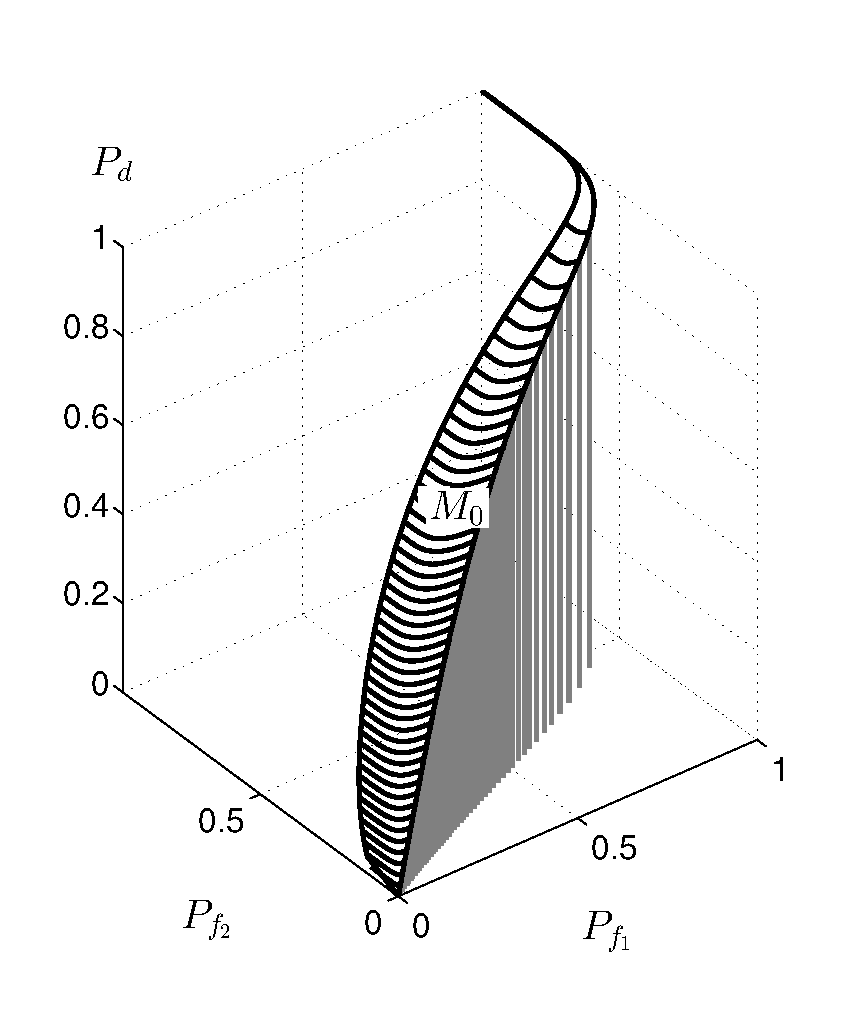
\includegraphics[width=12cm]{singleROC.eps}
\caption{Region that can be achieved by Neyman Pearson testing with $k_i \geq 0 (i=1, ..., M)$.}
\label{pic: surface for m0 gaussian}
\end{figure}
\newpage
\begin{figure}[!t]
\centering
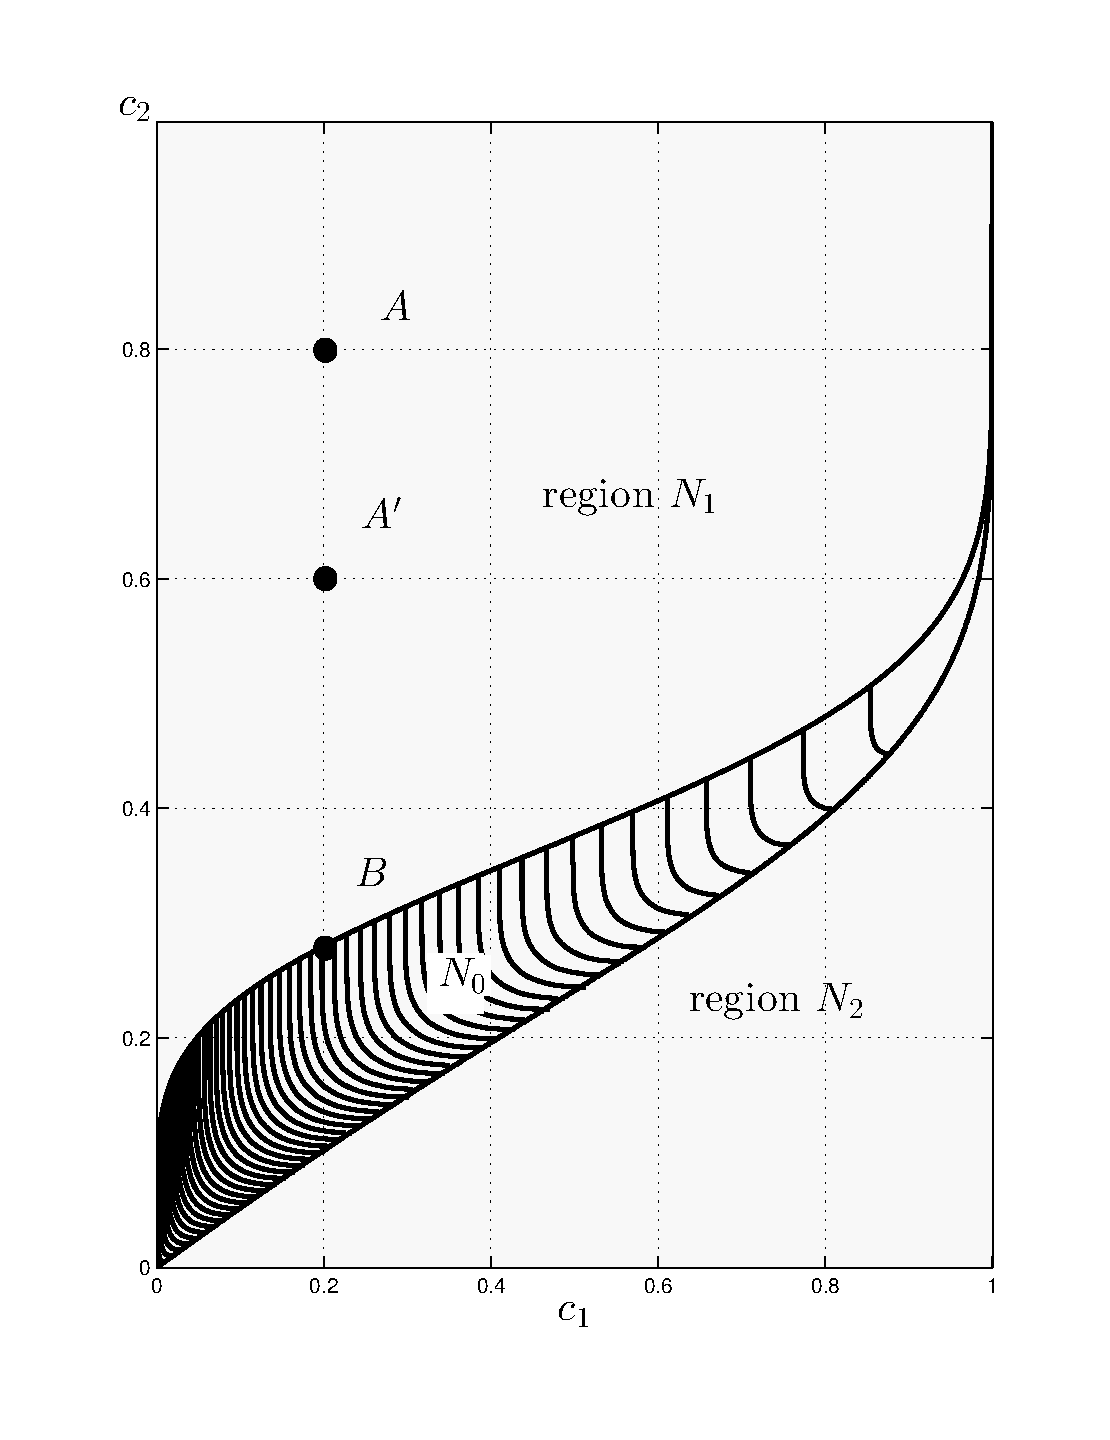
\includegraphics[width=12cm]{singlecontour.eps}
\caption{Region that can be achieved by Neyman Pearson testing with $k_i \geq 0 (i=1, ..., M)$.}
\label{pic: contour for m0 gaussian}
\end{figure}

\begin{figure}[!t]
\centering
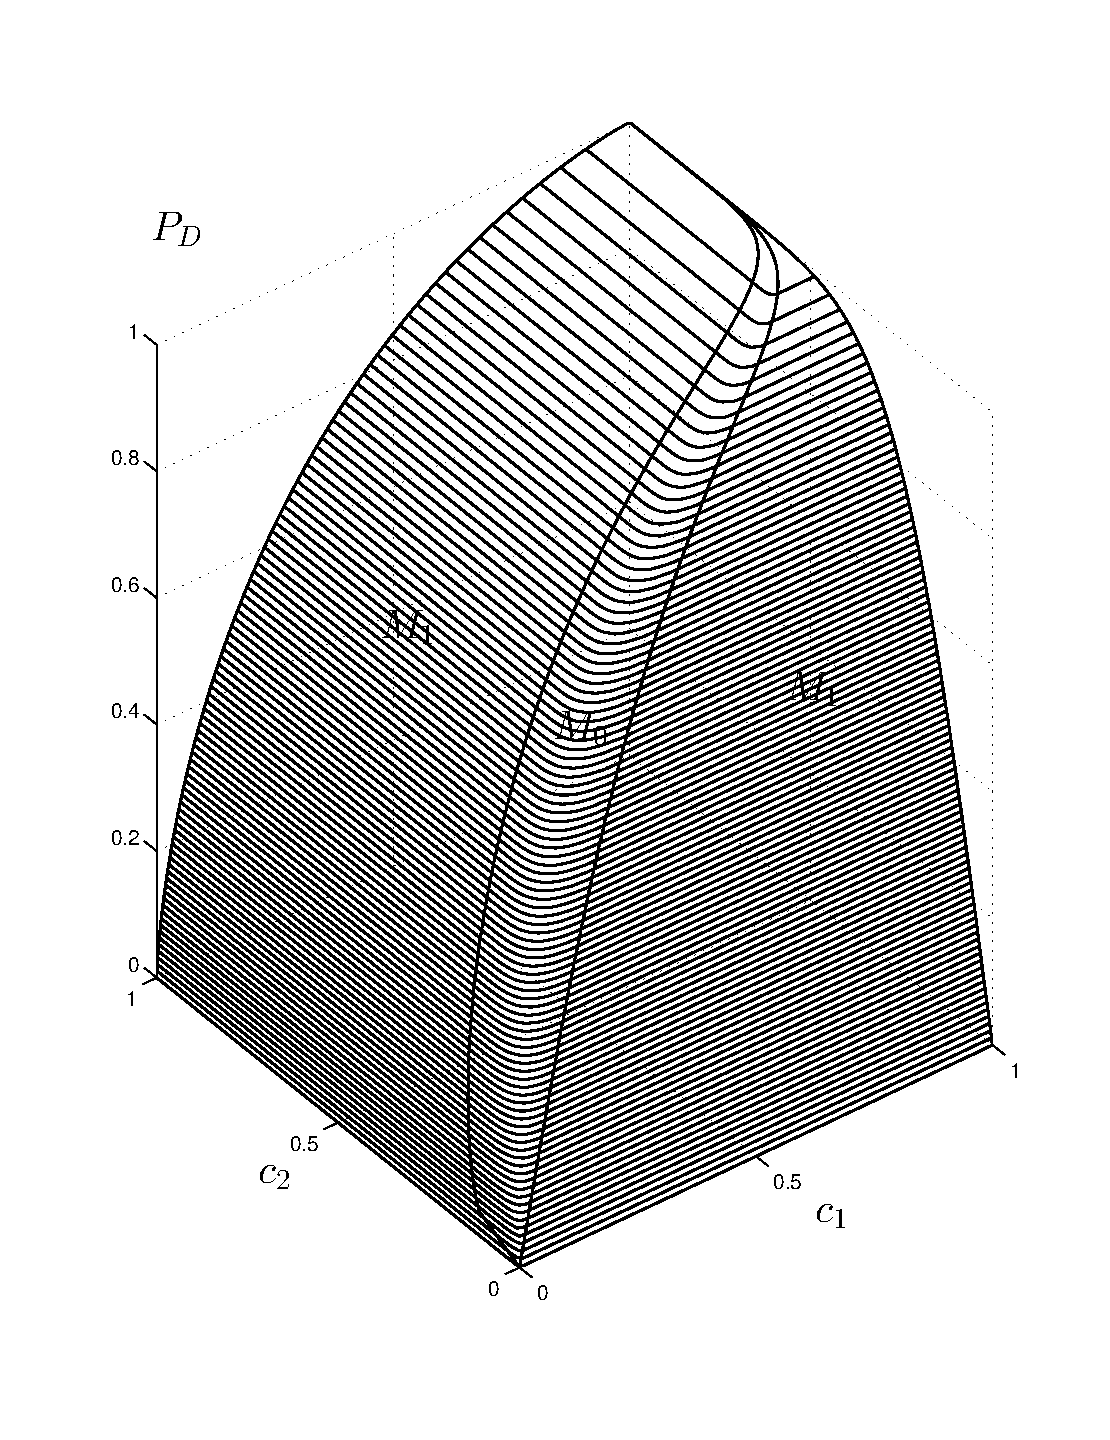
\includegraphics[width=12cm]{ROC2.eps}
\caption{The M-ROC surface for Gaussian Hypotheses.}
\label{pic: LJS}
\end{figure}

\begin{figure}[!t]
\centering
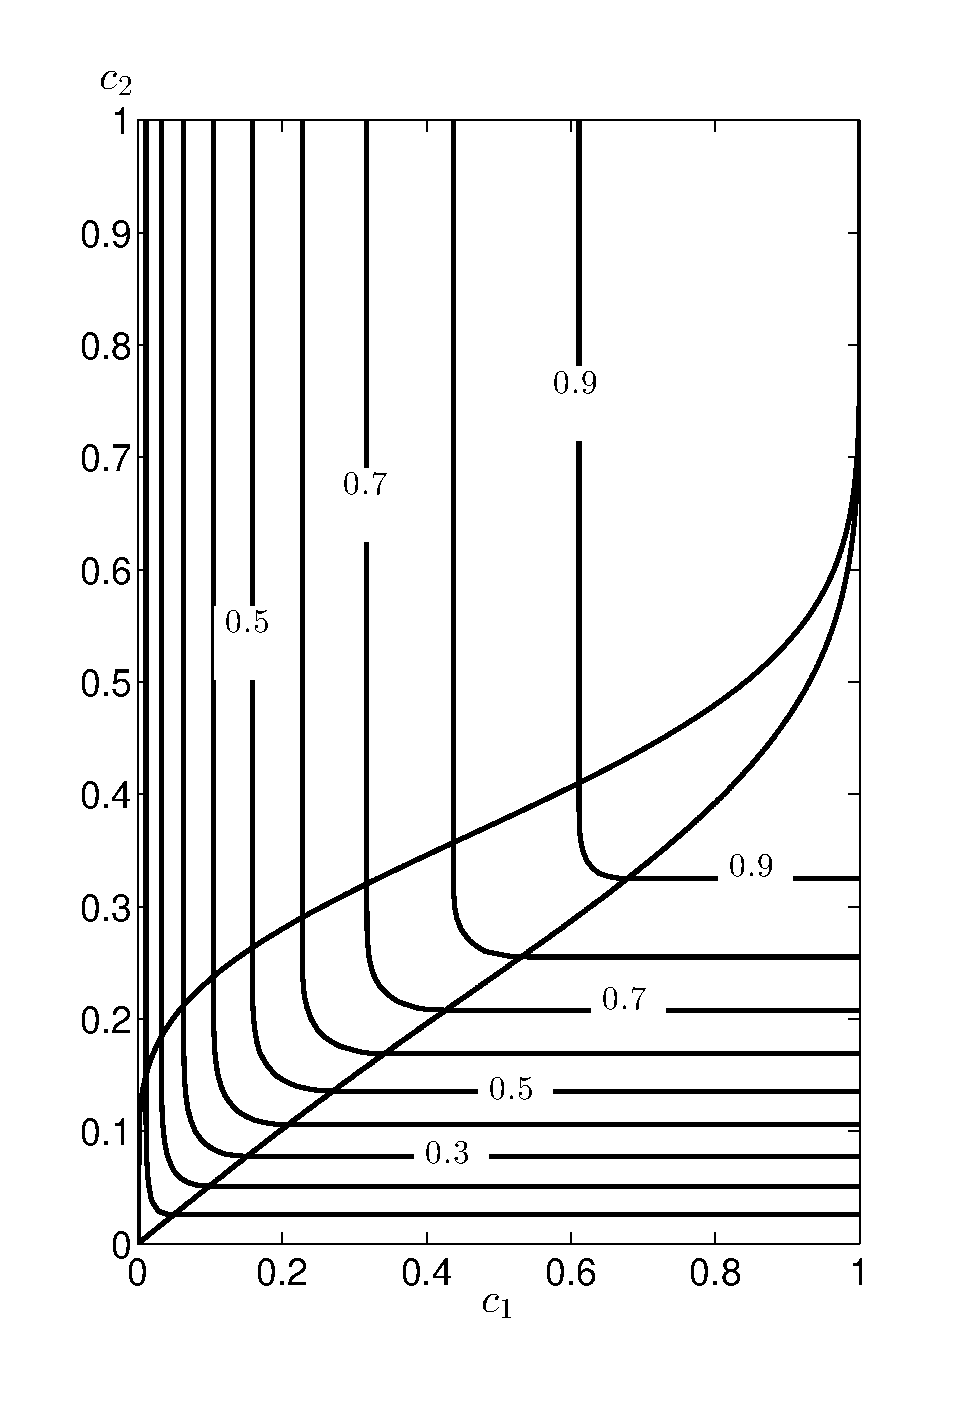
\includegraphics[width=12cm]{LJcontour.eps}
\caption{Contour for M-ROC surface.}
\label{pic: LJS contour}
\end{figure}


\begin{figure}[!t]
\centering
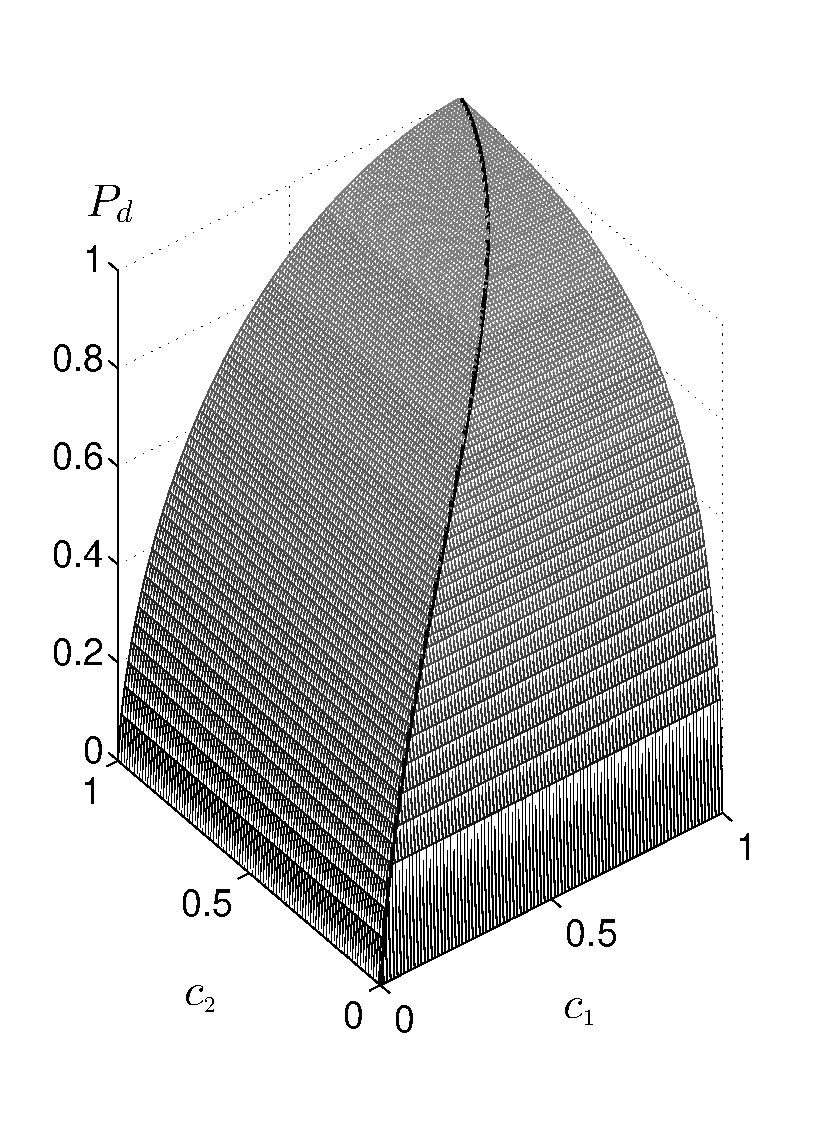
\includegraphics[width=12cm]{simu_chi2ROC.eps}
\caption{The M-ROC for the Chi-square example.}
\label{pic: LJS for chisquare}
\end{figure}


\begin{figure}[!t]
\centering
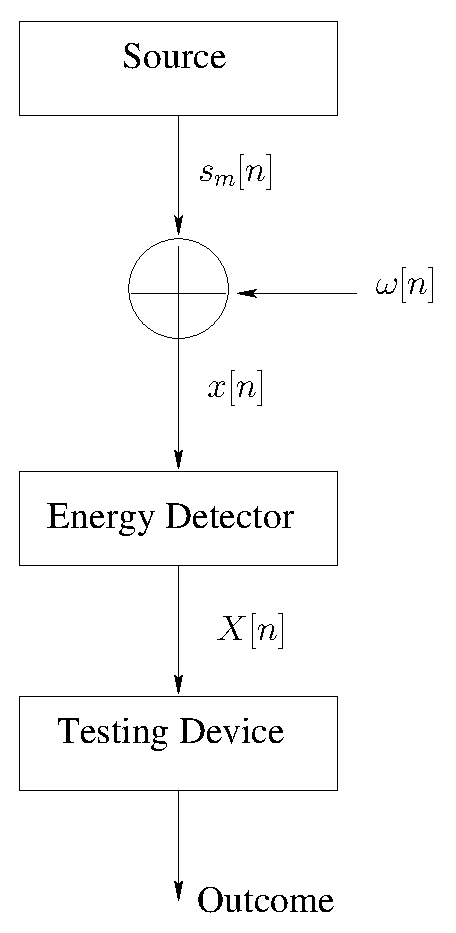
\includegraphics[width=8cm]{fig1.eps}
\caption{The Block Diagram for Energy Based Spectrum Sensing.}
\label{pic: block diagram}
\end{figure}

\begin{figure}[!t]
\centering
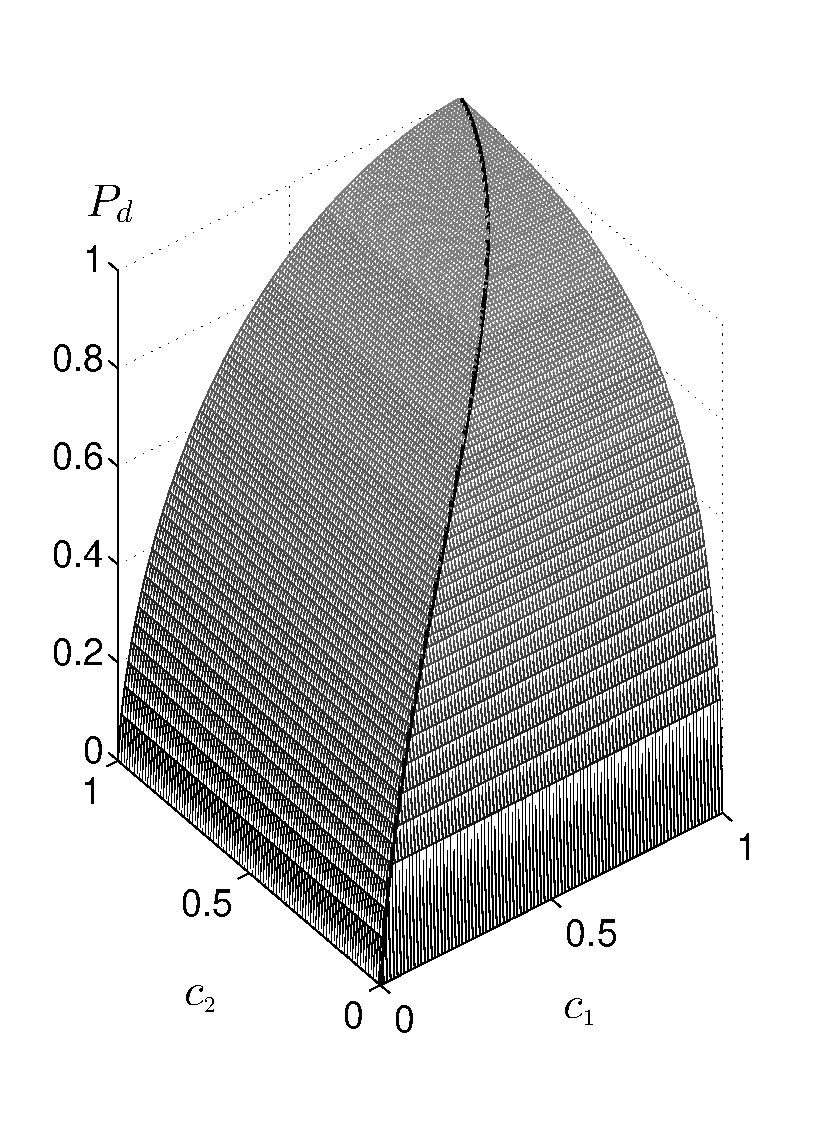
\includegraphics[width=12cm]{simu_chi2ROC.eps}
\caption{Analysis performance of MENP test for $\sigma_\omega^2=1$, $\sigma_{s_1}^2=0.1$ $\sigma_{s_2}^2 = 0.15$, $N=120$.}
\label{317}
\end{figure}

\begin{figure}[!t]
\centering
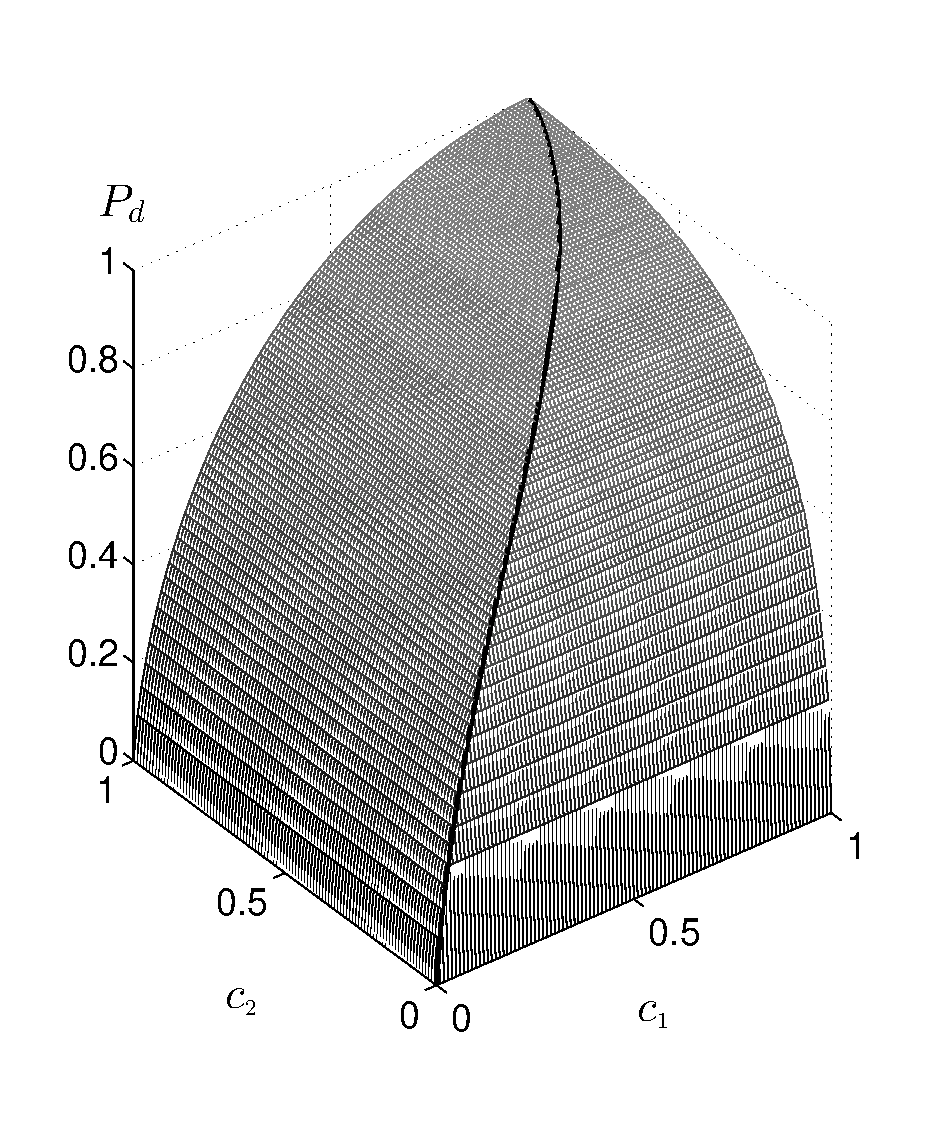
\includegraphics[width=12cm]{simu_c.eps}
\caption{Monte Carlo Simulation of MENP test for $\sigma_\omega^2=1$, $\sigma_{s_1}^2=0.1$ $\sigma_{s_2}^2 = 0.15$, $N=120$.}
\label{pic: simulation result}
\end{figure}

\end{spacing}
\end{document}
